\scanpage{34}
\mspage{1}
Special systems of five points on a complex sphere (more general\textsuperscript{ly} on a \deleted{\unsure{curve}} projective line over an algebraically closed field \(k\) \unsure{of} characteristic \(0\))

These are the systems \((\Sigma,K)\) with \(K\subset\Sigma\), \(\operatorname{Card}K=5\), and such that there exists a nontrivial automorphism of \((\Sigma,K)\) --- i.e. the group \inserted{\(G\)} of automorphisms of \((\Sigma,K)\) is not reduced \unsure{to|;} \(1\). We carry out the classification according to the structure of this group.

Let \(g\in G\) be of maximal order. We can identify \(g\) with a permutation of \(I\), and the discussion proceeds according to the structure of the latter. Note that \deleted{the order of \(g\ne1\) is} every automorphism of finite order of \(\Sigma\) \deleted{\(\unsure{\forall|\nu}\,g\) of order \(5\)} has exactly two fixed points, and that \deleted{\unsure{it is}} \inserted{if the order is \(\nu\)}, \(\mathbb Z/\nu\mathbb Z\) acts freely on \(\Sigma\setminus\Sigma^g\). This shows that
\[
K=K^g\amalg\text{orbits of order }\nu,\quad\text{hence }2\leq\nu\leq5.
\]
\margin{the action \unsure{is that|usual} of \(\mu_\nu\) on \(\widehat{\mathbb G_m}\)}

\textcircled{1} \(\nu=5\), then \(K\) is an orbit --- we may suppose that it is the orbit \(\mu_5(k)\) of \(\mu_5\) acting on \(\mathbb P^1_k\). The full group of automorphisms is \tikz[baseline=(d.base),x=.007cm,y=-.007cm,line cap=round,line join=round]{
\node (d) at (421,66) {$\mathbb D_5$};
\draw[line width=.5pt] (375,30)
 .. controls (393,4) and (444,7) .. (466,26)
 .. controls (493,48) and (489,97) .. (467,116)
 .. controls (443,139) and (398,139) .. (370,119)
 .. controls (344,102) and (341,65) .. (354,44);
}. Up to isomorphism, there is only one such case.

\margin{\unsure{Pentagonal|Pentagonal} structure on \(I\) (``pentagon'')}
\figure{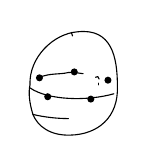
\begin{tikzpicture}[scale=.75,line cap=round,line join=round]
\draw (-.73,-.03) .. controls (-.75,.43) and (-.34,.84) .. (.08,.87)
 .. controls (.65,.93) and (.75,.45) .. (.75,-.05)
 .. controls (.77,-.58) and (.42,-.87) .. (-.05,-.88)
 .. controls (-.39,-.89) and (-.60,-.73) .. (-.68,-.53)
 .. controls (-.74,-.34) and (-.76,-.16) .. (-.73,-.03);
\draw (-.73,-.08) .. controls (-.43,-.29) and (.23,-.31) .. (.69,-.18);
\draw (-.60,.09) .. controls (-.36,.18) and (-.25,.14) .. (-.08,.18)
 .. controls (.01,.19) and (.09,.17) .. (.17,.16);
\draw (.38,.10)--(.42,.11)--(.44,.07);
\draw (.43,0)--(.43,-.03);
\draw (.59,.07)--(.61,.02);
\foreach \x/\y in {-.57/.09,.02/.19,.59/.05,-.43/-.23,.30/-.27}
 {\fill (\x,\y) circle(1.7pt);}
\draw (-.68,-.53) .. controls (-.47,-.58) and (-.25,-.60) .. (-.08,-.60);
\draw (-.03,.86)--(-.01,.80);
\end{tikzpicture}}

\textcircled{2} \(\nu=4\) then \deleted{\(K=\operatorname{Card}I^g=1\)} \inserted{\(K^g=\{P\}\)}, and \(I\setminus\{P\}\) is an orbit. We may suppose that it is \(\mu_4\), on which \(\mu_4\) acts, and \(P\) is a pole : \(\unsure{\infty|0}\). The full group of automorphisms is \(\mathbb Z/4\mathbb Z\simeq\mu_4(k)\).

The category of these configurations is equivalent to that of oriented squares.

\margin{``square pyramid''}
\figure{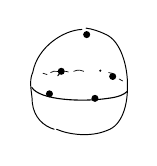
\begin{tikzpicture}[x=.0075cm,y=-.00818cm,line cap=round,line join=round]
\draw[line width=.35pt] (102,14)
 .. controls (71,15) and (27,41) .. (19,80)
 .. controls (11,96) and (18,112) .. (18,128)
 .. controls (21,151) and (37,164) .. (55,169);
\draw[line width=.35pt] (59,169)
 .. controls (79,177) and (115,182) .. (144,171)
 .. controls (171,163) and (179,130) .. (179,104)
 .. controls (180,70) and (167,32) .. (143,22)
 .. controls (132,17) and (119,13) .. (109,12);
\draw[line width=.4pt] (17,104)
 .. controls (31,124) and (102,127) .. (146,121)
 .. controls (163,119) and (172,116) .. (179,110);
\draw[line width=.25pt] (36,82) -- (43,84);
\draw[line width=.25pt] (49,81)
 .. controls (56,76) and (62,82) .. (69,78);
\draw[line width=.25pt] (74,79) -- (79,80);
\draw[line width=.25pt] (88,79)
 .. controls (96,76) and (101,77) .. (105,79);
\draw[line width=.25pt] (147,81) -- (153,82);
\draw[line width=.25pt] (165,91) -- (171,94);
\draw[line width=.35pt] (67,79)--(61,86);
\fill (133,78) circle[radius=.425pt];
\fill (110,22) circle[radius=1.275pt];
\fill (67,79) circle[radius=1.275pt];
\fill (154,87) circle[radius=1.275pt];
\fill (47,114) circle[radius=1.275pt];
\fill (124,121) circle[radius=1.275pt];
\end{tikzpicture}}

\textcircled{3} \(\nu=3\), Then \deleted{\(\unsure{\Sigma|K}_{\unsure{2}}\)} \(\operatorname{Card}K^g=2\), \inserted{hence \(K^g=\Sigma^g\),} and \(I\setminus K^g\) \inserted{\(=J\)} is an orbit,
\deleted{The group \unsure{as a whole is|of automorphisms}}
\inserted{which we may suppose to be \(\mu_3\).} The category of these configurations is equivalent : that of combinatorial triangles i.e. that \(\mathrm{Ens}(3)\) of sets \(J\) of cardinality \(3\).

To \(J\) we associate \(\Sigma_J\unsure{\deleted{\Sigma}|\deleted{g}\Omega|\deleted{G}\Omega}\) with \(J\cup P_J\) (\(P_J\subset\Sigma_J^{\unsure{g}}\) set of the two poles of \(\Sigma_J\) for \(1\)-\(1\) correspondence with the set \(\omega(\unsure{I|J})\) of orientations of \(J\), if \(\unsure{k|K}=\mathbb C\)). Group of automorphisms is \(\mathbb D_3\).

\margin{\unsure{Partition|A partition} \(2\) and \(3\) (in order of richness in symmetries)}
\margin{``bitetrahedron''}
\figure{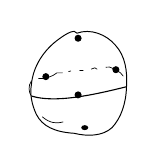
\begin{tikzpicture}[x=.00706cm,y=-.0080cm,line cap=round,line join=round]
\draw[line width=.35pt] (104,16)
 .. controls (128,8) and (157,18) .. (173,35)
 .. controls (191,52) and (195,77) .. (193,102)
 .. controls (192,128) and (183,151) .. (167,166)
 .. controls (150,180) and (122,180) .. (99,175)
 .. controls (64,173) and (42,164) .. (31,145)
 .. controls (23,130) and (19,113) .. (22,98)
 .. controls (25,68) and (45,42) .. (72,25)
 .. controls (86,16) and (100,9) .. (104,16);
\draw[line width=.4pt] (23,116)
 .. controls (64,127) and (130,115) .. (193,101);
\draw[line width=.25pt] (35,88)
 .. controls (46,89) and (60,85) .. (68,79)
 -- (78,79);
\draw[line width=.25pt] (89,77) -- (93,76);
\draw[line width=.25pt] (109,75) -- (115,75);
\draw[line width=.25pt] (130,73) -- (136,71) -- (140,73);
\draw[line width=.25pt] (156,70)
 .. controls (166,68) and (170,74) .. (174,75)
 .. controls (181,77) and (185,81) .. (187,84);
\draw[line width=.25pt] (42,149)
 .. controls (55,159) and (68,160) .. (79,157);
\draw[line width=.25pt] (22,92)..controls(16,99)and(17,110)..(22,116);
\fill (106,24) circle[radius=1.275pt];
\fill (48,85) circle[radius=1.275pt];
\fill (174,74) circle[radius=1.275pt];
\fill (106,114) circle[radius=1.275pt];
\fill (118,166) ellipse[x radius=1.275pt,y radius=.9pt];
\end{tikzpicture}}
\margin{33}
